\chapter{Obtención de geometría}

La reconstrucción tridimensional de una superficie es la construcción de un modelo que la representa. Se define una correspondencia entre los puntos del modelo y de la superficie real. En esta sección se presentan distintas técnicas y métodos que permiten la construcción automática de modelos, discutiendo distintas características según propiedades de la superficie a representar y de la tecnología utilizada. Un conjunto de puntos, también llamado nube de puntos, es la representación de una superficie utilizada por varias técnicas y dispositivos. Utilizando procesamientos de datos se puede obtener información adicional entre los puntos, como normales que identifiquen orientación de la superficie, y subgrupos de puntos que representan caras de una malla. La construcción del modelo se presenta en dos etapas, inicialmente obteniendo puntos de la superficie y luego procesando los datos para completar el modelo.

\section{Correspondencia}

\subsection{Calibración}

Al calcular coordenadas tridimensionales a partir de imágenes obtenidas por capturas de video se introducen errores propios del modelo (modelo \emph{pinhole}, modelo imaginario que utiliza una cámara) por ello es necesario hacer una corrección obteniendo una correspondencia entre el modelo real y el ideal, la calibración puede utilizarse como método para obtener la correspondencia mencionada. Luego de la calibración las coordenadas obtenidas son en dos dimensiones, corresponden a la proyección sobre el plano imagen, para completar las coordenadas tridimensionales en el modelo es necesario calcular la profundidad de cada punto, con este fin se utiliza el método de triangulación. El modelo ideal que se utiliza en las cámaras es el modelo \emph{pinhole}, éste se presenta para un caso básico, se considera que el centro de proyección $C$ coincide con el origen del sistema de coordenadas, y que $Z = f$ (plano imagen o plano focal).

\begin{figure}[H]
  \centering
    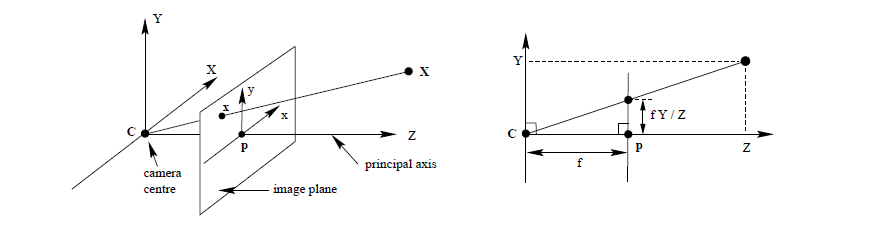
\includegraphics[width=0.8\textwidth]{./Cap6_reconstruccion/pinhole.png}
  \caption{Geometría de cámara pinhole. $C$ es centro de la cámara y $p$ el punto principal}
  \label{fig:Calib-Pinhole}
\end{figure}

Un punto en el espacio $ \vec{X}=(X,Y,Z)^T$ se corresponde con el punto $X$ en el plano imagen, dado por la intersección del rayo que pasa por el centro de cámara y el punto $\vec{X}$ con el plano imagen, el punto $(X,Y,Z)^T$ es mapeado con $(\frac{f_X}{Z}, \frac{f_Y}{Z}, f)^T$ en el plano imagen.
$(X, Y, Z)^T \to (\frac{f_X}{Z}, \frac{f_Y}{Z},f)^T$ se considera que el centro de coordenadas del plano imagen coincide con el punto principal $P$.
El centro de proyección $C$ es el centro de la cámara o centro óptico.
Proyección central utilizando coordenadas homogéneas:
Considerando la representación de los puntos como vectores homogéneos se expresa la proyección central como una correspondencia lineal entre las coordenadas homogéneas:

\[
\begin{pmatrix}
X \\ Y \\ Z \\ 1
\end{pmatrix}
\to
\begin{pmatrix}
f_X \\ f_Y \\ Z
\end{pmatrix}
=
\begin{pmatrix}
f & 0 & 0 & 0 \\
0 & f & 0 & 0 \\
0 & 0 & 1 & 0 \\
\end{pmatrix}
\begin{pmatrix}
X \\ Y \\ Z \\ 1
\end{pmatrix}
\]

Dados $\vec{X} = (X,Y,Z,1)^T$ y $\vec{x} =(x,y,z)^T$ la correspondencia utilizando el método pinhole es:
$\vec{x}=P\vec{X}$

Siendo
\[
P = 
\begin{pmatrix}
f & 0 & 0 & 0 \\
0 & f & 0 & 0 \\
0 & 0 & 1 & 0 \\
\end{pmatrix}
\]

Considerando el caso general en el cual el centro de coordenadas del plano de proyección no coincide con el punto principal $P$ (las coordenadas de $P$ son $(p_x,p_y)^T$ ) la correspondencia es dada según:
$(X,Y,Z)^T \to (\frac{fX}{Z} + p_x, \frac{fY}{Z} + p_y, f)^T$

\[
\begin{pmatrix}
X \\ Y \\ Z \\ 1
\end{pmatrix}
\to
\begin{pmatrix}
f_X + Z * p_x \\ f_Y + Z * p_y \\ Z
\end{pmatrix}
=
\begin{pmatrix}
f & 0 & p_x & 0 \\
0 & f & p_y & 0 \\
0 & 0 & 1 & 0 \\
\end{pmatrix}
\begin{pmatrix}
X \\ Y \\ Z \\ 1
\end{pmatrix}
\]

\[
K =
\begin{pmatrix}
f &   & p_x & \\
  & f & p_y & \\
  &   & 1   & \\
\end{pmatrix}
\]

$K$ es la matriz de calibración, y se utilizará para obtener la correspondencia de cada punto según:
$x = K [I|0] X$
(siendo $[I|0]$ la matriz identidad sumado a una columna de ceros)
$X = (X,Y,Z,1)^T$ coordenadas espaciales considerando que el centro de la cámara coincide con el origen de coordenadas del sistema Euclidiano.
$x = (x, y, z)$ coordenadas que se buscan determinar.
En caso de considerar que el centro de coordenadas de la cámara no coincide con el origen de coordenadas del sistema Euclidiano es necesario utilizar una traslación y rotación para lograr esta correspondencia\cite{LibroCompGrafica3}.

\subsection{Método de triangulación}
Este método determina las coordenadas $(x,y,z)$ de un punto utilizando la posición del punto obtenida en las perspectivas de dos proyecciones dadas.
Los centros de perspectiva y planos de proyección son conocidos\cite{PresUnivYonsei}.
Escena con dos dimensiones (2D)

\begin{figure}[H]
  \centering
    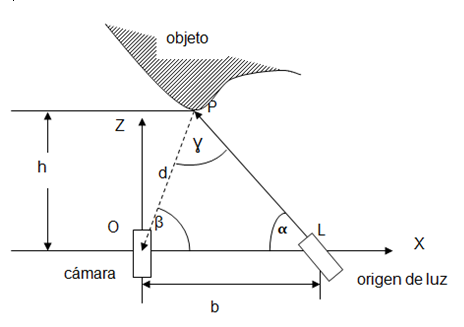
\includegraphics[width=0.65\textwidth]{./Cap6_reconstruccion/triangulacion.PNG}
  \caption{Diagrama con propiedades trigonométricas para escena 2D.}
  \label{fig:Triangulacion}
\end{figure}

Este método tiene como objetivo calcular la distancia $d$ de la cámara al punto $P$ a partir de los datos: ángulos $\hat\alpha$, $\hat\beta$ y la distancia $b$ entre el proyector y la cámara.
El ángulo $\hat\alpha$ y la distancia $b$ son dados por la calibración de la escena.
El ángulo $\hat\beta$ esta dado por la geometría de la proyección.

\[
\left.
\begin{array}{l}
\frac{d}{\sin (\hat\alpha)} = \frac{b}{\sin (\hat\gamma)} 	\\
\gamma = \pi - (\alpha + \beta)								\\
\sin (\pi - \gamma) = \sin (\gamma)
\end{array}
\right \rbrace
\frac{d}{\sin(\gamma)} = \frac{b}{\sin(p - \gamma)} = \frac{b}{\sin(\alpha + \beta)} \Rightarrow d = b . \frac{\sin(a)}{\sin(\alpha + \beta)}
\]

Las coordenadas cartesianas quedan determinadas por:
\[
X_o = d. \cos (\beta)
\]
\[
Z_o = d. \sin (\beta) = h
\]

Escena con tres dimensiones (3D)

\begin{figure}[H]
  \centering
    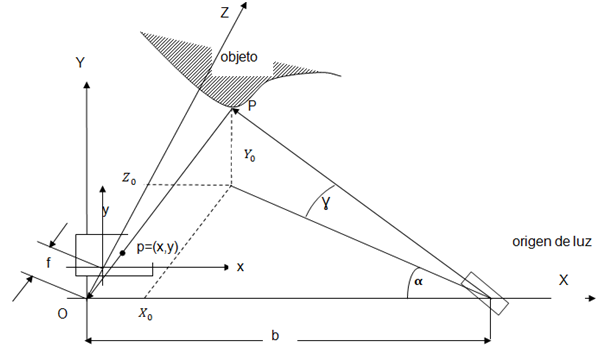
\includegraphics[width=0.65\textwidth]{./Cap6_reconstruccion/triangulacion-2.PNG}
  \caption{Diagrama con propiedades trigonométricas para escena 3D.}
  \label{fig:Triangulacion2}
\end{figure}

Se asume $Z = f$, $f$ plano en el cual se proyecta el punto $P(X_o,Y_o,Z_o)$, obteniendo como resultado de la proyección el punto $p(x,y)$.
El centro óptico del proyector está situado en el eje $X$.
Se considera realizada una pre-calibración en la cual se define:
\[
P = (x,y), \quad \frac{X_o}{x} = \frac{Z_o}{f} = \frac{Y_o}{y} = k \to (k_x,k_y,k_f)
\]
\[
k_f = \tan (\alpha)(b - kx)
\]

Por trigonometría:
\[
\tan (\alpha) = \frac{Z_0}{(b - X_0)} \Rightarrow Z_0 = \tan (\alpha) (b - X_0) \quad k = \frac	{b * \tan (\alpha)}{f + x * \tan (\alpha)}
\]
\[
X_o = \frac{x * b * \tan (\alpha)}{f + x * \tan (\alpha)}, \quad Yo = \frac{y * b * \tan (\alpha)}{f + x * \tan (\alpha)},\quad Zo = \frac{f * b * \tan (\alpha)}{f + x * \tan (\alpha)}
\]

Los métodos que resuelven obtener la geometría de una escena tridimensional sin tener contacto físico se pueden clasificar como activos o pasivos. [4]
Los métodos pasivos son aquellos en los que no es necesario utilizar luz adicional a la luz ambiente.

\subsection{Visión estéreo}

Es un método pasivo para obtener la estructura tridimensional de una escena, se utiliza el método de triangulación sin intervención de luz auxiliar, la correspondencia es establecida entre dos o más imágenes.
Los algoritmos que utilizan este método son clasificados basados en diferencias de la geometría de la imagen, distintas estrategias para resolver la correspondencia entre puntos y en las diferentes estructuras computacionales utilizadas\cite{StereoReview}.
Se realiza un pre proceso de las imágenes para identificar las principales características que se utilizarán, luego se define qué tipo de correspondencia se utilizará.
La principal desventaja de este método es que en caso de oclusión, hay regiones que no tienen correspondencia en las dos imágenes por lo tanto no se puede establecer la correspondencia de puntos, finalmente no se puede resolver el problema de correspondencia para estas regiones.
Las variantes que influyen en la geometría de la imagen son, ejes ópticos\footnote{Ver glosario.} paralelos o no, paradigma binocular o multiocular.
La correspondencia entre una o más vistas de la escena se puede realizar basada en distintas estrategias que son separate area o features.
\begin{itemize}
   \item \emph{separate area}, basada en correlación del brillo, intensidad, se utilizan patrones de brillo aplicados a un pixel y sus vecinos (utiliza principio de localidad), diferencias en la perspectiva de la imagen o cambios en luminosidad absoluta de la escena puede generar errores.
   \item \emph{features}, las características usadas para la correspondencia son aristas, puntos o segmentos dadas por cambios de intensidad de la imagen, esta estrategia es más estable  ante variedad de luminosidad absoluta y en la práctica correspondencia es más rápida.
\end{itemize}
La geometría convencional estéreo tiene un par de cámaras y los ejes ópticos son paralelos entre sí, y perpendiculares a la línea base (dada por los dos centros ópticos de las cámaras).

\begin{figure}[H]
  \centering
    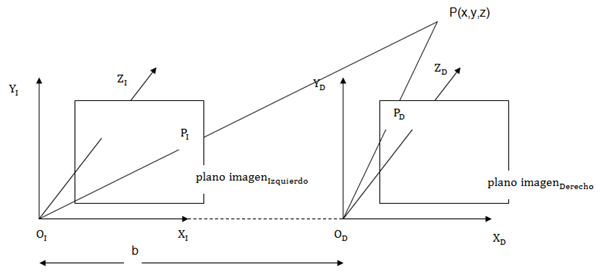
\includegraphics[width=0.5\textwidth]{./Cap6_reconstruccion/stereo.PNG}
  \caption{}
  \label{fig:Stereo}
\end{figure}

\subsection{Luz estructurada}

El método basado en la técnica de luz estructurada consiste en proyectar distintos patrones sobre la superficie a modelar, luego se realizan capturas de las proyecciones, analizando las deformaciones de los patrones proyectados se obtiene información de la posición (coordenadas tridimensionales), orientación y textura de la superficie\cite{SLightPatterns}.
Los patrones a utilizar en este método pueden ser variados se clasifican en cuatro tipos: punto (singled scanned dot), línea (slit line), grilla (grid) y matriz de puntos (dot matrix).
Dependiendo del tipo de objeto y superficie a escanear se puede tener problemas de oclusión, baja reflexión y puntos reflejados fuera del alcance de la cámara, como consecuencia, hay pérdida de puntos proyectados que no tienen proyección en el plano imagen.
Estos problemas se pueden solucionar utilizando patrones codificados adecuados. Se distinguen tres grupos de patrones clasificados según: dependencia temporal, propiedades de la luz proyectada y discontinuidad de profundidad de la superficie proyectada\cite{SLightCorrespondence}.
\begin{itemize}
   \item Dependencia  temporal:
   \begin{itemize}
	\item Estática, el patrón es limitado para escenas estáticas, son necesarias proyecciones de varios patrones distintos. El movimiento de cualquier objeto de la escena mientras se realiza la obtención de los patrones proyectados producirá un error de correspondencia.
	\item Dinámica, los objetos en la escena se pueden mover, se utiliza un único patrón de proyección.
   \end{itemize}
   \item Propiedades de la luz proyectada:
   \begin{itemize}
	\item Binaria, cada uno de los puntos del patrón tiene dos posibles valores codificados con 0 y 1 respectivamente. Este valor representa opacidad y transparencia, ausencia o presencia de la luz proyectada en el objeto.
	\item Escala de grises, cada punto del patrón tiene asociado un valor de gris que representa el nivel de trasparencia (o nivel de opacidad) del punto para la luz proyectada. Son necesarios dos pasos, primero se obtiene una imagen de la escena iluminada con la misma luz (sin variar la intensidad), luego se obtiene la referencia de luz necesaria para cancelar el efecto de reflejo de la superficie (depende directamente del tipo de superficie). La necesidad de estos dos pasos contribuye a que este patrón también sea clasificado como estático.
	\item Color, cada punto del patrón es asociado con un valor de tono. Los tonos deben ser bien diferenciados para alcanzar una segmentación eficiente. Este tipo de patrones son limitados por el color de la escena, si presenta objetos de colores altamente saturados se producen pérdidas de regiones en el paso de segmentación que luego provoca errores en la decodificación.
   \end{itemize}
   \item Discontinuidad en profundidad de la superficie proyectada:
   \begin{itemize}
	\item Periódica, la codificación se repite periódicamente a lo largo del patrón. Esta  técnica se utiliza para reducir el número de bits que codifican el patrón, como limitante la profundidad del objeto no puede ser mayor que la mitad de la longitud del período.
	\item Absoluta, cada columna o fila del patrón proyectado tiene una única codificación, no sufre dependencia de discontinuidad de profundidad.
   \end{itemize}
\end{itemize}

   
\section{Sensores}
\subsection{Kinect}

Kinect es un dispositivo que se puede adicionar a la consola  Xbox360 de Microsoft. El objetivo de este dispositivo es permitir que el usuario interactúe con la consola utilizando solo el movimiento de su cuerpo. Para lograr eso, Kinect aplica distintas técnicas de procesamiento de imágenes, considerando ubicaciones, posturas y distancias. El hardware de Kinect no consiste tan solo de una cámara, sino que tiene adicionalmente un emisor de infrarrojo, que en base a la deformación del haz de luz determina la distancia de cada punto de la imagen capturada. Posteriormente, combina la información visual para tener una noción bastante precisa de los movimientos del usuario. A mediados del 2011 fue presentada una interfaz de programación gratuita que permite utilizar Kinect de forma directa en aplicaciones no licenciadas y para diferentes propósitos, no solo el de los video juegos.

\begin{figure}[H]
  \centering
    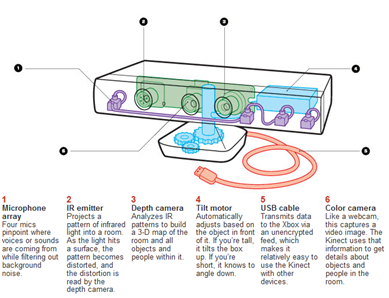
\includegraphics[width=0.5\textwidth]{./Cap6_reconstruccion/kinect.PNG}
  \caption{Componentes de un sensor Kinect}
  \label{fig:Kinect}
\end{figure}

Para el análisis de las deformaciones de los rayos y construir el mapa de profundidad, Kinect utiliza la previamente mencionada técnica de Luz Estructurada. Mediante el sensor infrarrojo con el que viene equipado, se proyectan los patrones de luz por toda la escena y se analizan las distorsiones mediante la cámara de profundidad
También se cuenta con una cámara convencional para analizar objetos o personas en la escena y la detección de colores.
En cuanto a los usos específicos orientados a la reconstrucción tridimensional de objetos, el proyecto KinectFusion, actualmente esponsoreado por Microsoft, logra muy buenos resultados\cite{KinectFusion}.

\section{Procesamiento de nube de puntos}

Utilizando técnicas de structured light, stereo, laser, sensores infrarojos o kinect se obtienen miles de puntos, es necesario simplificar este modelo con el objetivo de eliminar redundancia, y aumentar la velocidad en el procesamiento de los datos. Un problema adicional al tamaño de la información obtenida es que comúnmente se introduce información errónea (ruido), para superar este problema se realiza un suavizado en el procesamiento de la nube de puntos (en \cite{PCloudSimplify} se presentan distintos métodos para simplificar y aproximar superficies 3D).

Las heurísticas utilizadas se pueden clasificar como\cite{PntCloud}:
\begin{itemize}
   \item Clustering methods, consta en obtener subgrupos de la nube de puntos, cada subgrupo se remplaza por un conjunto de puntos representativos en él. Los subgrupos se pueden construir de dos formas, una utilizando un enfoque incremental, en el cual los subgrupos (clusters) son creados por construcción de menor a mayor (region-growing), otro enfoque es el jerárquico en el cual se subdivide utilizando una estrategia top-down.
   \item Iterative simplification, se recorren iterativamente los puntos de la nube generando contracciones de pares de puntos a un nuevo punto, se evalúa el error introducido que genera la contracción comparándolo con el error que se obtendría al contraerse con un punto vecino (el error se calcula utilizando mínimos cuadrados), se elije la contracción que introduce menor error al sistema, la finalización se puede dar por haber logrado la cantidad de puntos deseada o por superar una cota de error a introducir en el sistema.
   \item Particle simulation, se generan nuevos puntos que sustituyen la nube de puntos original, inicialmente se genera conjuntos de partículas que se mueven aleatoriamente en la superficie, luego utilizando algoritmo de point – repulsión se definen en las zonas que hay mayor colisiones.
\end{itemize}

En la sección Tratamiento de malla se detallan los algoritmos utilizados en nuestra solución.
Luego de simplificar la nube de puntos se construye un modelo tridimensional a partir de ella, las estructuras obtenidas son mallas de poliedros, particularmente son muy usadas las mallas triangulares, la razón principal es la simplicidad de los algoritmos que dibujan triángulos, esto permite que sean implementados fácilmente en hardware, otro beneficio de los triángulos es que cualquier polígono con más de tres caras puede representarse con un conjunto de triángulos\cite{PCloudTriangle}.

\section{Tratamiento de malla}

Los dispositivos de captura de información tridimensional estudiados entregan la información en forma de nube de puntos (ref a Kyle, kinect  y Sensores del chino). Es por ello que previo a la manipulación de la información tridimensional, es necesario procesar dicha nube de puntos para convertirla a formatos más manejables, como por ejemplo mallas triangulares.
Un típico procesamiento de malla, ya estudiado e implementado en bibliotecas como VcgLib\cite{VCGLib} o CGAL\cite{CGAL}: dada una nube de puntos de entrada, realizar un sub-muestreo y suavizado de la misma, calcular las normales en cada punto de la nube y finalmente, aplicar algoritmos de reconstrucción de malla.

\begin{figure}[H]
  \centering
    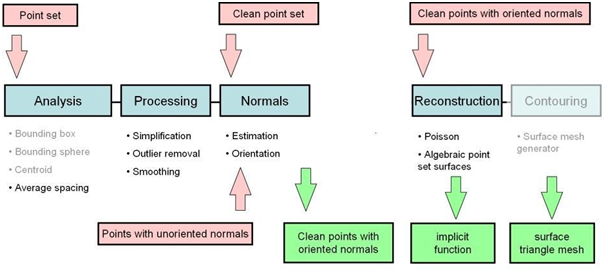
\includegraphics[width=0.5\textwidth]{./Cap6_reconstruccion/malla-flow.png}
  \caption{Típico flujo para el procesamiento de nubes de puntos (fuente: CGAL\cite{CGAL})}
  \label{fig:Mesh-CGAL}
\end{figure}

Para la implementación de este modulo, se utilizaron algoritmos incluidos en VcgLib. Para visualizar y evaluar los resultados esperados se utilizo la aplicación de código abierto para la manipulación de mallas tridimensionales en diferentes formatos MeshLab Error: Reference source not found. Particularmente, se utilizaron los algoritmos de muestreo Poisson-disk para reducir y normalizar los puntos de la malla inicial, Normal Extrapolation para el cálculo de normales y reconstrucción de superficies de Poisson para la reconstrucción de la malla final.

\subsection{Muestreo Poisson-disk}

El muestreo o sorteo de variables aleatorias es una técnica utilizada para una gran variedad de aplicaciones graficas, incluyendo dibujado (rendering), procesamiento de imágenes y de geometrías.
Particularmente, el muestreo Poisson-disk se utiliza para ubicación aleatoria de objetos en mundos artificiales, algoritmos de texturas procedurales y procesamiento de geometrías o mallas. Esta técnica genera conjunto de puntos con las siguientes propiedades: puntos suficientemente juntos, pero con la restricción de no estar más próximos unos de otros que una distancia mínima R predeterminada.

\begin{figure}[H]
  \centering
    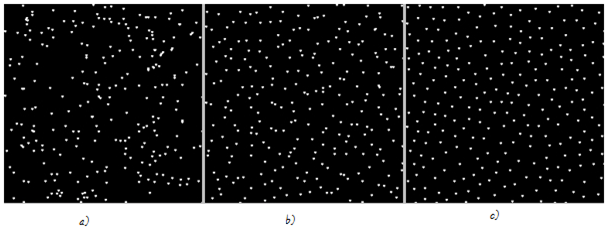
\includegraphics[width=0.5\textwidth]{./Cap6_reconstruccion/malla-poisson.png}
  \caption{a) Posición x e y generadas aleatoriamente. b) Imagen dividida en celdas. Puntos aleatorios generados en cada celda. c) Muestreo Poisson-disk en 2 dimensiones}
  \label{fig:Mesh-Poisson}
\end{figure}

En líneas generales, este algoritmo genera puntos alrededor de los ya existentes en la muestra, y valida si pueden ser agregados al conjunto final en caso de no violar la regla de la mínima distancia a los vecinos. Se genera una grilla en 2 o 3 dimensiones dependiendo del escenario de aplicación, en la cual cada celda contendrá al final del proceso a lo sumo un punto. Una grilla adicional es utilizada para realizar búsquedas rápidas, y dos conjuntos de puntos son mantenidos durante el procesamiento para poder diferenciar los que han sido generados y los que aún necesitan procesamiento.
La implementación de VcgLib utilizada recibe 3 parámetros:
\begin{itemize}
	\item La cantidad de puntos en la muestra. En este caso el radio o parámetro de cercanía es calculado en base a este parámetro.
	\item El radio, que es a su vez utilizado para calcular el tamaño de la muestra optimo en base a la malla inicial.
	\item Sub muestreo: indica si la muestra de Poisson es un subconjunto de la muestra inicial o si se deberán generar nuevos puntos aleatoriamente.
\end{itemize}

\begin{figure}[H]
  \centering
    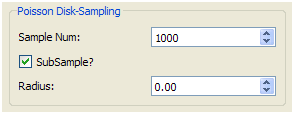
\includegraphics[width=0.5\textwidth]{./Cap6_reconstruccion/malla-poissongui.png}
  \caption{Configuracion de parámetros del alrogirtmo Poisson-disk}
  \label{fig:Mesh-PoissonGui}
\end{figure}

\subsection{Reconstrucción de normales}

Este algoritmo computa las normales en cada elemento de un conjunto de puntos sin la necesidad de explorar la conectividad de los triángulos. Por ello es que es muy útil para objetos tridimensionales sin información de caras (faces).
Se detalla un pseudocódigo del método:

Figura: planos tangentes

\subsubsection{Paso 1: Identificar los planos tangentes para aproximar localmente la superficie y estimar así los vectores normales}
Para cada vértice:
	\begin{itemize}
		\item Calcular el centro geométrico (centroide) del plano tangente en el punto como el promedio de los K puntos más cercanos.
		\item Calcular la normal asociada al centro geométrico. Se utiliza la matriz de covarianza en el punto contemplando los mismos K vecinos más cercanos de la muestra y los valores y vectores propios de la matriz de covarianza. Finalmente, ordenando los vectores propios, la estimación del vector perpendicular corresponde al vector propio de menor valor. Este método es conocido como PCA (Principal Component Analysis).
	\end{itemize}

\subsubsection{Paso 2: construir grafo donde cada punto está conectado a los K vecinos más cercanos (grafo de Riemannian)}
Se crea un grafo en cuyos nodos se guardan todas las aristas a los K vecinos más cercanos. Cada arista se pesa con el valor absoluto del producto escalar de la normal en el punto con la normal en cada uno de los K vecinos:
   $$fabs(nodoActual->normal . K\_Vecinos[n]->normal)$$
\subsubsection{Paso 3: calcular el árbol de expansión mínimo (MST) sobre el grafo de Riemannian y recorrerlo para orientar las normales}
Dado un grafo conexo, no dirigido, con sus aristas con un peso asignado, se llama árbol de expansión mínimo al sub-grafo con forma de árbol que conecta todos los nodos con un peso total mínimo. Contiene todos los nodos del grafo inicial. El grafo de entrada es el construido en el paso enterior y se utiliza el algoritmo de Kruskal, uno de los varios algoritmos que resuelven el problema de encontrar un árbol de expansión mínima de un grafo (referencias).
Una vez construido el MST, lo único que se hace es recorrer el árbol en orden y corregir el sentido de los vectores normales (multiplicando por -1.0f) en caso de ser necesario. La condición para efectuar dicha corrección se basa en el ángulo del nodo siendo inspeccionado versus todas las direcciones de las normales de los vecinos conectados a dicho nodo.

\begin{figure}[H]
  \centering
    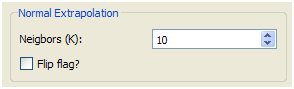
\includegraphics[width=0.5\textwidth]{./Cap6_reconstruccion/malla-normalextrapolation.png}
  \caption{Configuracion de parámetros para reconstruccion de normales}
  \label{fig:Mesh-Extrapolation}
\end{figure}

\subsection{Reconstrucción de malla de Poisson}

Finalmente, para reconstruir la malla a partir de la nube de puntos y sus normales se utiliza el algoritmo de Reconstrucción de Poisson.
Se computa una función indicador $\chi$ en 3 dimensiones definida de la siguiente forma:

$$
\left\{ \begin{array}{rl}
 \chi = 1 & \mbox{ si puntos dentro del modelo} \\
 \chi = 0 & \mbox{ si puntos fuera del modelo}
       \end{array} \right.
$$

Luego, se obtiene una reconstrucción de la superficie mediante la extracción de la ISO-surface (superficie de nivel en 3 dimensiones) al nivel apropiado.
La clave está en que hay una estrecha relación entre los puntos orientados (con sus normales) de la muestra y la función indicador de la muestra. Específicamente el gradiente de la función indicador es un espacio de vectores que valen cero casi en todo el espacio excepto en puntos cercanos a la superficie, donde es igual al vector normal a la superficie.
Es por eso que puntos orientados, pueden ser vistos como muestras del gradiente de la función indicador del modelo tridimensional en cuestión. Y es por este mismo motivo que el problema de reconstrucción de una malla puede ser visto como un problema de Poisson estándar: computar la función escalar $F$ cuyo Laplaciano (o divergencia del gradiente) se iguala a la divergencia del espacio de vectores de las normales.

\begin{figure}[H]
  \centering
    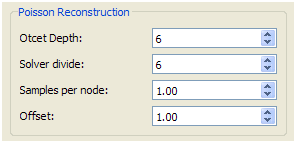
\includegraphics[width=0.5\textwidth]{./Cap6_reconstruccion/malla-poissonreconstruction.png}
  \caption{Configuracion de parámetros para reconstruccion de malla de Poisson}
  \label{fig:Mesh-Normals}
\end{figure}

\subsection{Pruebas y resultados}

Para validar el correcto funcionamiento de esta técnica utilizando los tres algoritmos descritos, utilizamos una malla inicial de 5021 vertices y 9608 caras triangulares. Cabe destacar que si bien se ha mencionado que la malla de entrada debe ser simplemente una nube de puntos, se pueden utilizar mallas con caras, solo que estas serán ignoradas e incluso removidas de la malla de salida del primer paso del procesamiento (Poisson-disk sampling).
Luego de experimntar con varios juegos de datos iniciales durante varias ejecuciones del procesamiento, se fijaron de manera personalizada para la malla de entrada algunos parámetros clave. Dado que la muestra inicial tiene alrededor de cinco mil puntos, elegimos cinco mil como cantidad de muestras para el algorimso de Poisson-disk. Luego, para la extrapolación de normales se utilizaran $K=15$ vecinos para la toma de decisiones locales de aproximación. 
La aplicación de estos algoritmos resultó ser lo esperado, en términos estructurales de cada malla procesada en cada uno de los paso. No se llego a procesar mallas de ambientes tridimensionales escaneados para luego ser mapeados con la herramienta.


\begin{table}
\begin{center}
\begin{tabular}{|l||cc|} \hline
	Fase & Vértices & Caras \\
	Nube inicial & 5021 & 9608 \\
	Luego Poisson-disk & 1776 & 0 \\
	Luego Extrapolación Normales & 1776 & 0 \\
	Luego de Poisson-recontruction & 1959 & 3910 \\ \hline
\end{tabular}
\caption{Comparación de estructura de mallas de entrada y salida en cada fase}
\end{center}
\end{table}

\begin{figure}[H]
  \centering
    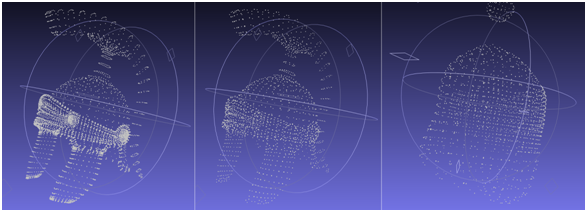
\includegraphics[width=0.8\textwidth]{./Cap6_reconstruccion/malla-nubepuntos.png}
  \caption{1) Nube de puntos inicial con 5021 vértices. 2) Resultado de muestreo Poisson-disk con 1776 vértices. 3) Luego de extrapolar normales y reconstruir la malla con 1959 vértices y 3910 caras.}
  \label{fig:Mesh-Results}
\end{figure}
 
Se observaron buenos tiempos computacionales de respuesta. Si bien la malla utilizada no es de un tamaño considerable, estamos hablando de algoritmos de orden relativamente alto.
